
\documentclass{article}
\usepackage{polski}
\usepackage{mathtools}
\usepackage{tikz}
\usepackage{float}
\usetikzlibrary{automata, positioning, arrows}
\tikzset{
->, % makes the edges directed
node distance=2.5cm, % specifies the minimum distance between two nodes. Change if necessary.
every state/.style={thick, fill=gray!10}, % sets the properties for each ’state’ node
initial text=$\epsilon$, % sets the text that appears on the start arrow
}


\title{Zadanie 8. z 1. listy zadań z JFTT}
\author{Michał Kallas}

\begin{document}

\maketitle

\section{Treść zadania}
Skonstruuj NFA rozpoznający język tych słów nad $\{0, 1\}^{*}$ które jako liczba w systemie dwójkowym dzielą się przez 5,
przy czym liczba jest wczytywana począwszy od najmniej znaczącego bitu.

\section{Rozwiązanie}
Zacznijmy od skonstruowania NFA działającego analogicznie do tego zadanego, ale wczytującego liczby w odwrotnej
kolejności, czyli \textbf{począwszy od najbardziej znaczącego bitu}.

W naszym automacie chcemy akceptować liczby podzielne przez 5. Zauważmy, że dana liczba albo dzieli się przez 5, albo
nie dzieli się z resztą 1, 2, 3 lub 4. To oznacza, że każdą liczbę możemy zaprezentować przez pryzmat tego jaką zwraca resztę z
dzielenia przez 5.

W takim wypadku nasz automat będzie składał się z 5 stanów: $\{q_0, q_1, q_2, q_3, q_4\}$. $q_0$
oznacza resztę z dzielenia wynoszącą 0, a więc będzie to nasz stan akceptujący.

Zauważmy, że czytając liczby począwszy od najbardziej znaczącego bitu, przy przeczytaniu każdej kolejnej cyfry
następuje przesunięcie bitowe w lewo aktualnej liczby oraz dodanie na jej koniec(jako najmniej znaczący bit) nowej
cyfry. Czyli, jeśli liczba $k = a \bmod{5}$, to:
$$kb = (2a + b) \bmod{5}$$

$kb$ oznacza konkatenację ciągu bitów $k$ z bitem $b$.\\

Na podstawie tej obserwacji możemy skonstruować naszą funkcję przejścia:
$$\delta(q_a, b) = q_{(2a + b) \bmod{5}}$$

Teraz możemy skonstruować automat:

\begin{figure}[H]
    \centering
    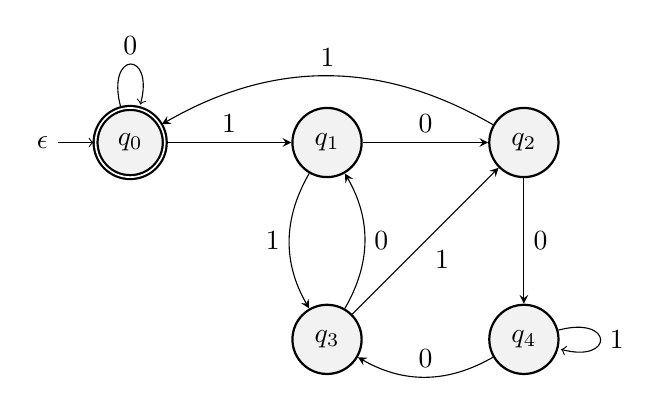
\begin{tikzpicture}
        \node[state, initial, accepting] (q0) {$q_0$};
        \node[state, right of=q0] (q1) {$q_1$};
        \node[state, right of=q1] (q2) {$q_2$};
        \node[state, below of=q1] (q3) {$q_3$};
        \node[state, below of=q2] (q4) {$q_4$};

        \draw[-stealth] (q0) edge[loop above] node{0} (q0)
              (q0) edge[above] node{1} (q1)
              (q1) edge[above] node{0} (q2)
              (q1) edge[left, bend right] node{1} (q3)
              (q2) edge[above, bend right] node{1} (q0)
              (q2) edge[right] node{0} (q4)
              (q3) edge[below right] node{1} (q2)
              (q3) edge[bend right, right] node{0} (q1)
              (q4) edge[loop right] node{1} (q4)
              (q4) edge[above, bend left] node{0} (q3)
              ;

    \end{tikzpicture}
\end{figure}

Na podstawie tego automatu, możemy stworzyć taki, który będzie wczytywał liczbę w odwrotnej kolejności, czyli od
najmniej znaczącego bitu. W tym celu obrócimy strzałki w powyższym automacie. Nie musimy zamieniać stanu początkowego
z akceptującym, bo to ten sam stan. Nie trzeba dodawać $\epsilon$-przejść, bo jest tylko jeden stan akceptujący w
powyższym DFA.

\begin{figure}[H]
    \centering
    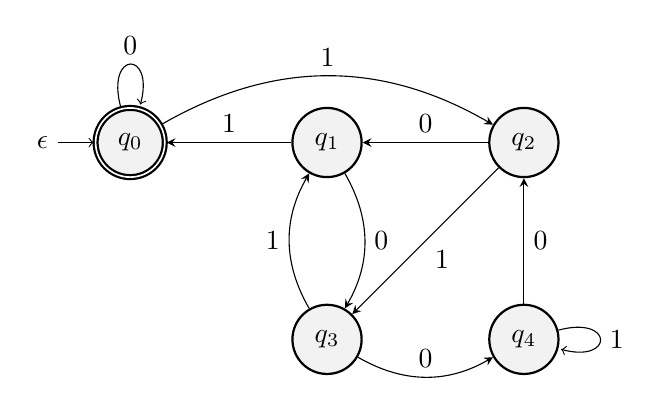
\begin{tikzpicture}
        \node[state, initial, accepting] (q0) {$q_0$};
        \node[state, right of=q0] (q1) {$q_1$};
        \node[state, right of=q1] (q2) {$q_2$};
        \node[state, below of=q1] (q3) {$q_3$};
        \node[state, below of=q2] (q4) {$q_4$};

        \draw[-stealth] (q0) edge[loop above] node{0} (q0)
              (q1) edge[above] node{1} (q0)
              (q2) edge[above] node{0} (q1)
              (q3) edge[left, bend left] node{1} (q1)
              (q0) edge[above, bend left] node{1} (q2)
              (q4) edge[right] node{0} (q2)
              (q2) edge[below right] node{1} (q3)
              (q1) edge[bend left, right] node{0} (q3)
              (q4) edge[loop right] node{1} (q4)
              (q3) edge[above, bend right] node{0} (q4)
              ;

    \end{tikzpicture}
\end{figure}

W ten sposób otrzymaliśmy szukany NFA.

\end{document}
